\section{Sistemas de recomendação}

Sistemas de recomendação são ferramentas computacionais e técnicas usadas para
produzir recomendação de itens úteis a um usuário \cite{mahmood2009improving}.
Sendo assim, um sistema de recomendação pode ser usado em diversos contextos,
desde melhorar a experiência de usuário a até mesmo melhorar a taxa de vendas
em uma aplicação comercial. Além disso, um sistema de recomendação também pode
ser usado para recomendar uma grande gama de itens, como filmes e livros
\cite{ricci2011introduction}. Para realizar a tarefa de recomendação, duas abordagens distintas podem ser usadas,
recomendação não-personalizadas e personalizadas.

Recomendações não-personalizadas são aquelas que não usam nenhuma informação do
usuário para realizar a recomendação. Exemplo de estratégias assim podem ser
visto em sites de música que apresentam a lista das 10 músicas mais
ouvidas. Já recomendações personalizadas são aquelas que usam as avaliações já
realizadas por um usuário sobre um item para criar uma função preditiva que irá avaliar itens que ainda não foram
avaliados pelo usuário e então recomendar aqueles que possuem maior valor
apresentado pela função preditiva. A Figura \ref{fig:modelo_recomendacao} mostra
o processo para realizar uma recomendação baseado em conteúdo.

\begin{figure}[h]
  \centering
  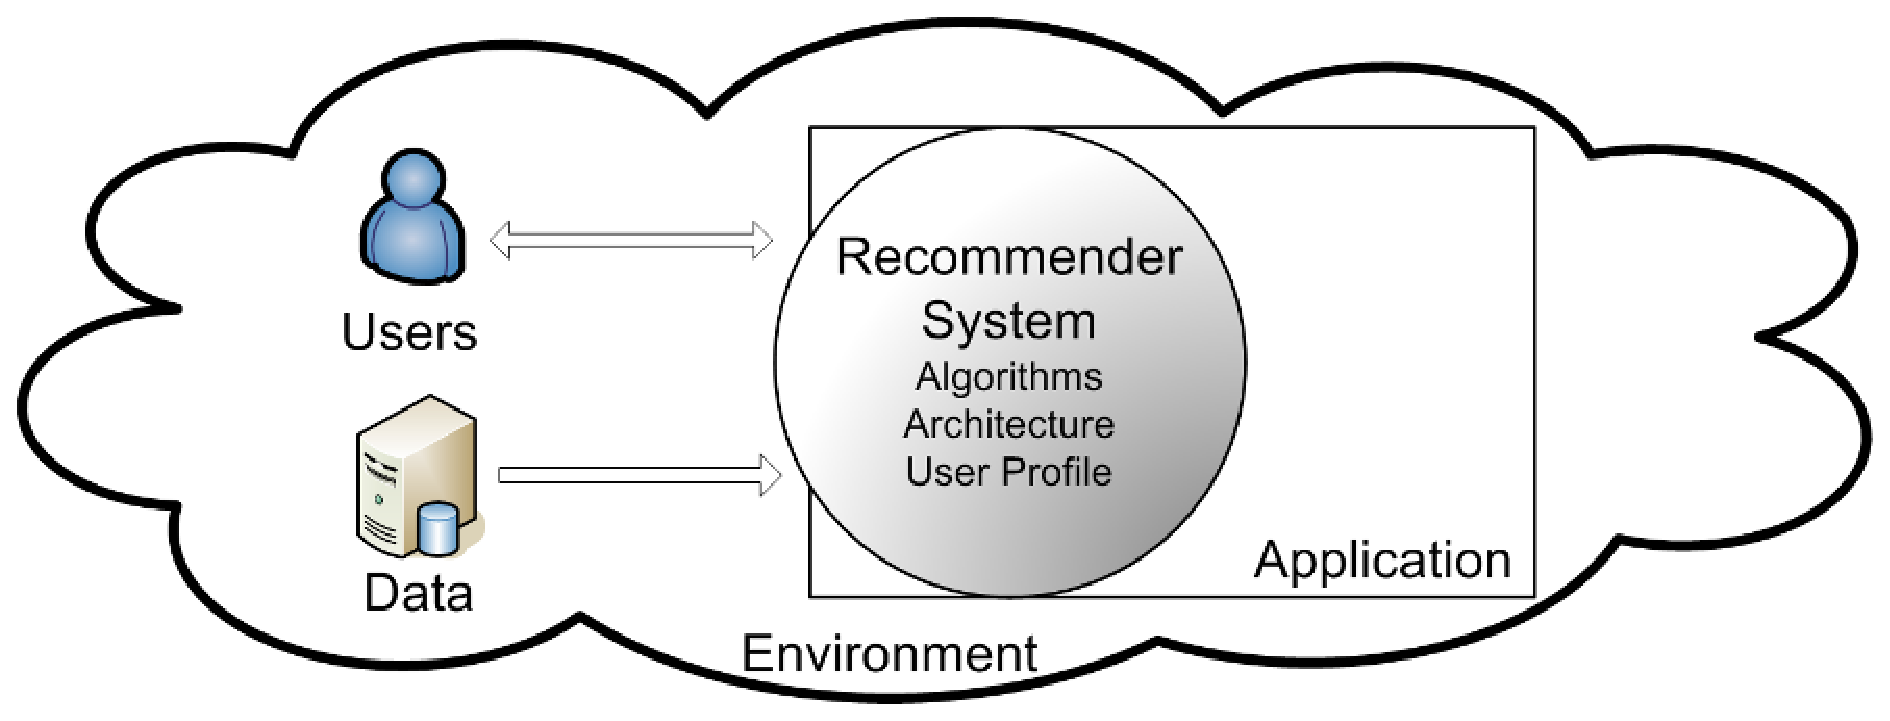
\includegraphics[width=0.9\textwidth]{figuras/recommender_model.eps}
  \caption{Modelo para criação de um sistema de recomendação personalizado \cite{picault2011get}}
  \label{fig:modelo_recomendacao}
\end{figure}

Pode-se ver na Figura \ref{fig:modelo_recomendacao} que as principais entradas
para um sistema de recomendação são os usuários do mesmo e os dados relacionados
a este mesmo usuário. No que tange o sistema de recomendação em si, pode-se
observar fatores importantes no design do mesmo, como o perfil do usuário, o
algoritmo de recomendação ou estratégia a ser usada e a infra-estrura a ser
usada. Além disso, nenhum sistema de recomendação está imune do contexto no qual
o usuário irá interagir com o sistema.

Vale considerar que o perfil do usuário e a estratégia de recomendação usadas
são bastante dependentes um do outro. O perfil do usuário é o item que o
identifica unicamente no sistema, como por exemplo, uma lista dos itens já
avaliados pelo usuário. Sendo assim, características dos itens, números de itens
avaliados e a forma como o perfil do usuário é modelado são aspectos
fundamentais para a seleção de uma estratégia de recomendação, pois dependendo
da configuração desses atributos, algumas estratégias
de recomendação devem ser descartadas \cite{picault2011get}.

\subsubsection{Estratégias de recomendação}

Com o conjunto de dados definidos, pode-se então escolher uma estratégia de
recomendação adequada. Para agrupar tais estratégias, considerou-se taxinomia de
alguns autores, como por exemplo \cite{burke2007hybrid}. As recomendações
descritas a seguir foram as que se mostraram mais presentes nas taxinomias
estudadas.

\begin{itemize}
    \item \textbf{Estratégias baseadas em conteúdo: } São aquelas que buscam
        recomendar itens similares ao que usuário já avaliou. A similiraridade
        dos itens é estimada pelos atributos que compõem um dado item no
        sistema. O fluxo de uma estratégia baseada em conteúdo pode ser vista na
        Figura \ref{fig:recomendacao_conteudo}

        \begin{figure}[h]
            \centering
            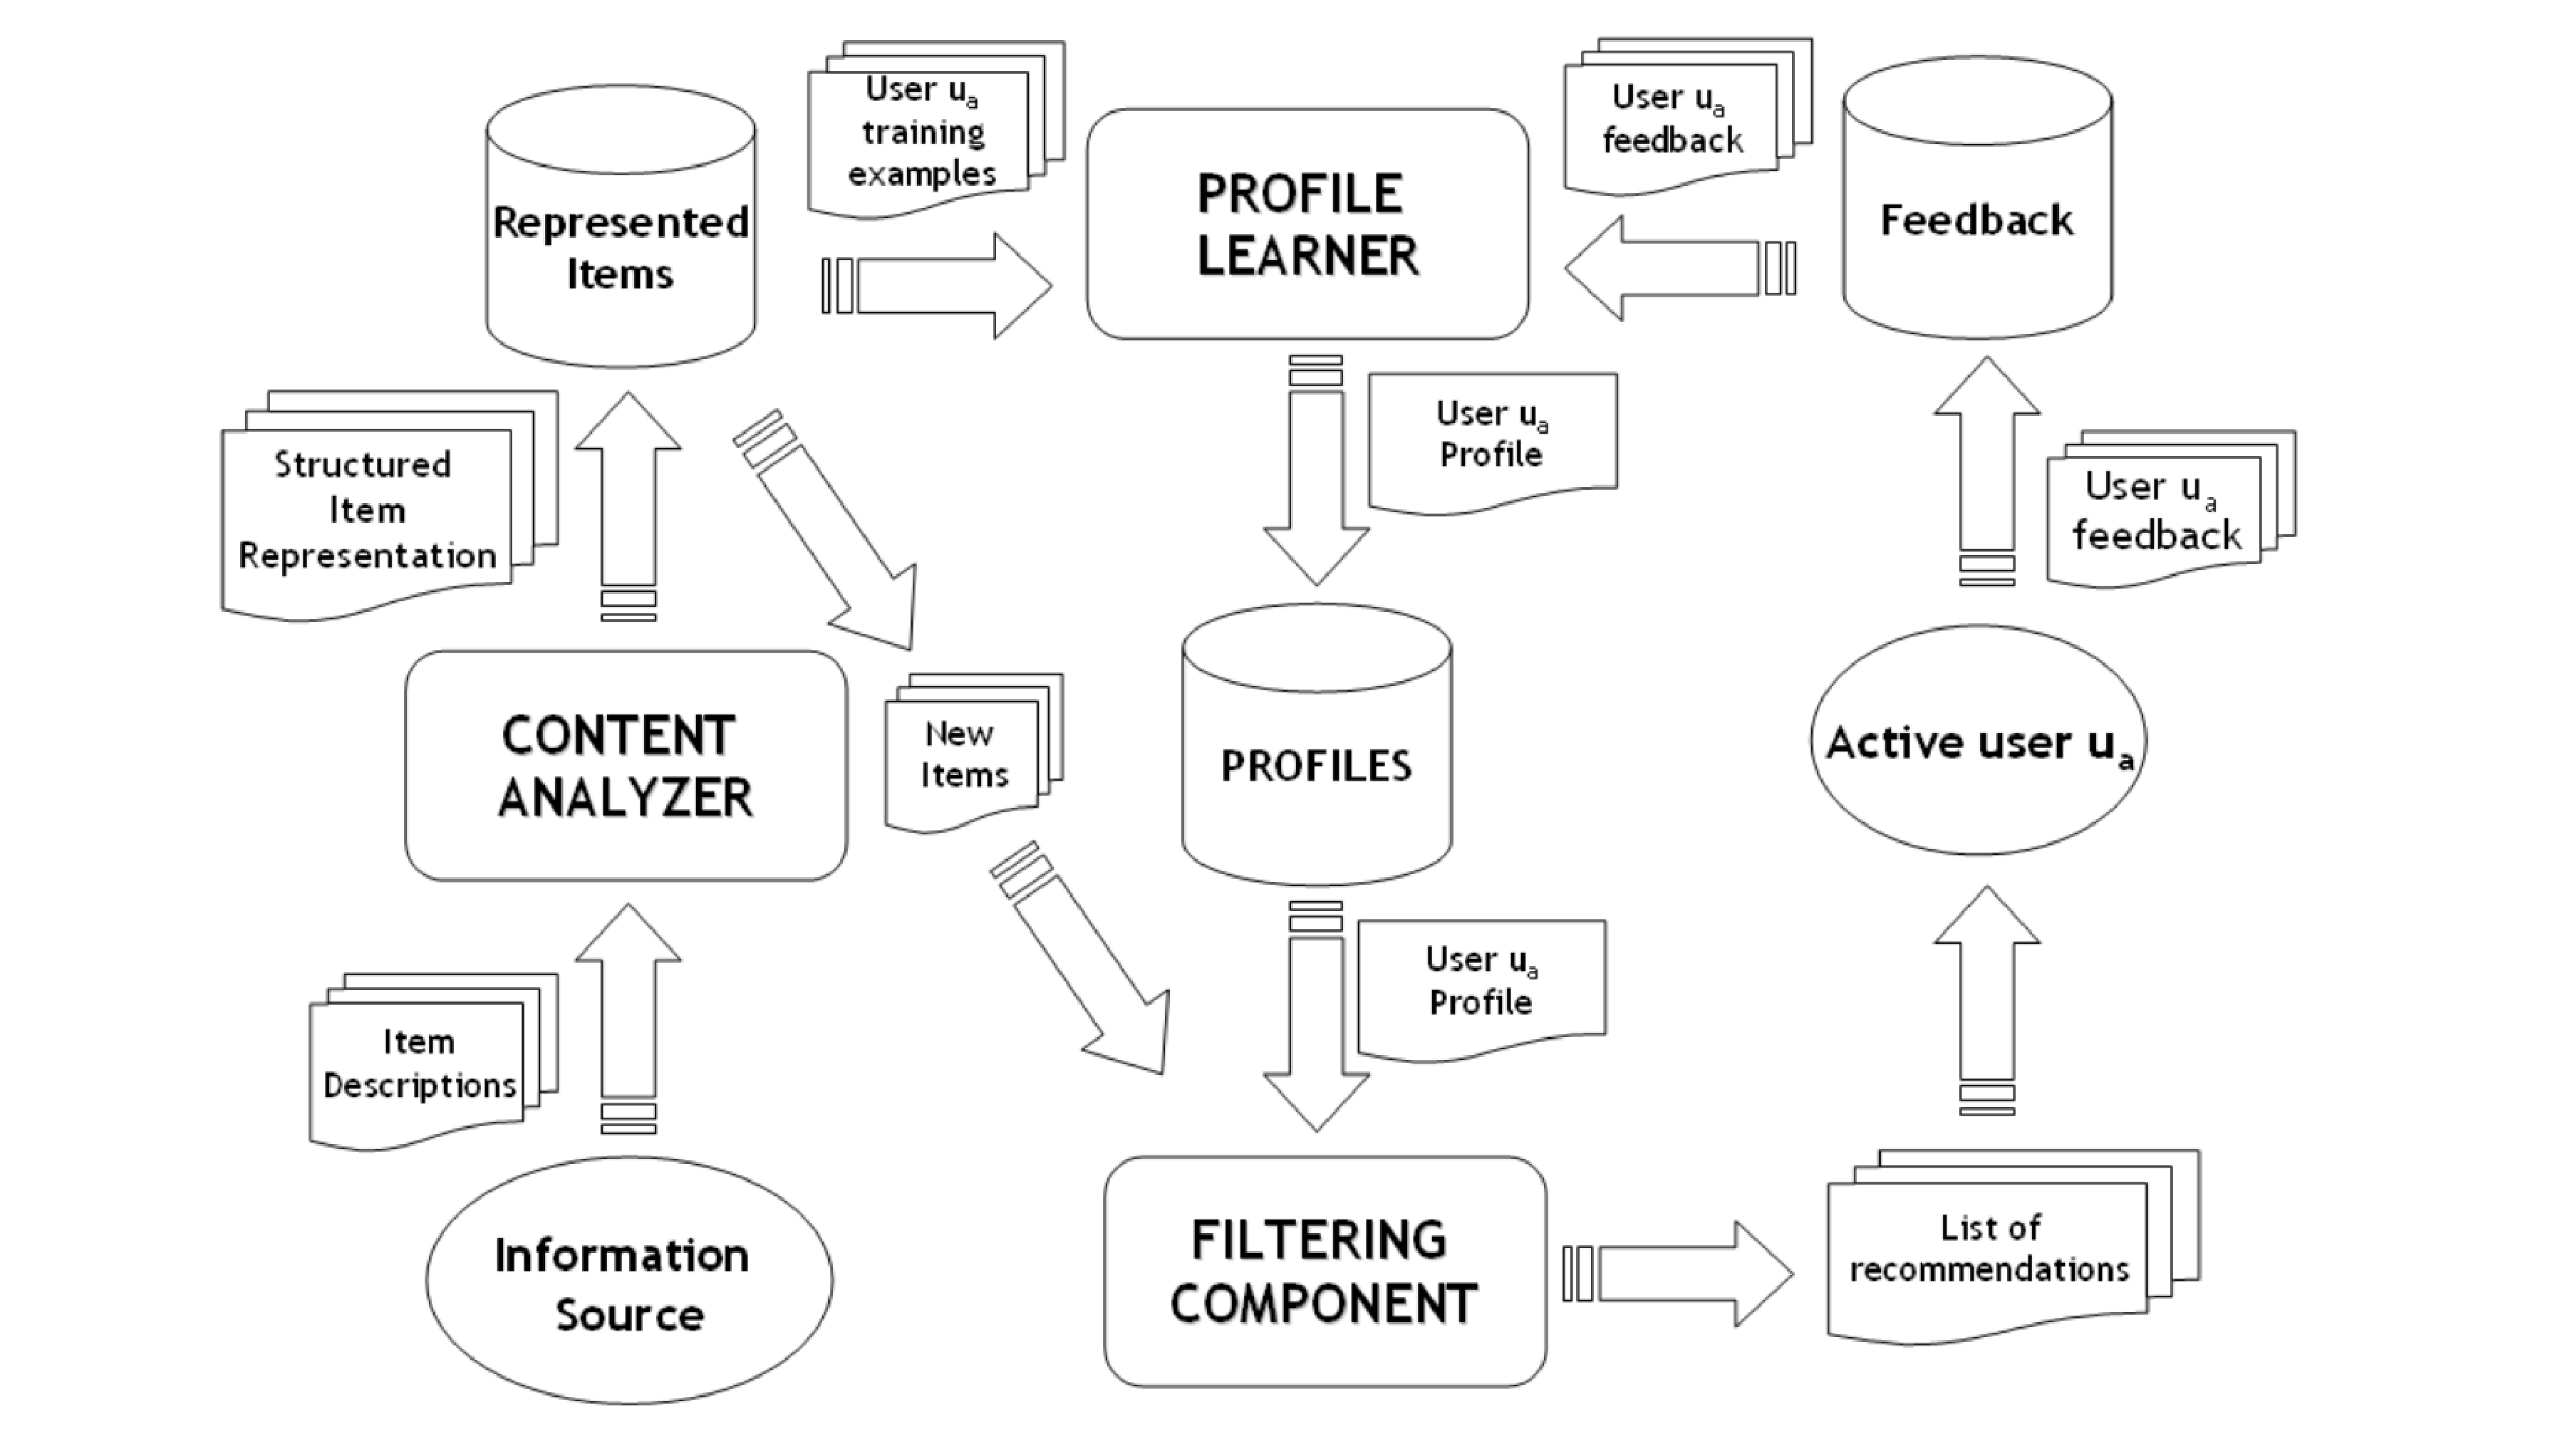
\includegraphics[width=0.9\textwidth]{figuras/recomendacao_conteudo}
            \caption{Fluxo para construção de um sistema de recomendação por
            conteúdo \cite{lops2011content}}
            \label{fig:recomendacao_conteudo}
        \end{figure}

        Pode-se ver pela Figura \ref{recomendacao_conteudo} que uma recomendação
        por conteúdo se baseia fortemente em alguns itens chave. O
        \textit{Content Analyser} é a parte do sistema de recomendação que
        transforma os itens avaliados pelo usuário em entradas válidas pelo
        algoritmo, ou seja, seleciona os atributos escolhidos do mesmo. O
        \textit{Profile Learner}, têm-se o parte que de fato cria o perfil do
        usuário, sendo que este item pode ser desde uma lista de atributos mais
        frequentes no itens avaliados pelo usuário ou até mesmo um modelo gerado
        por aprendizado de máquina, capaz de aproximar os gostos de um usuário.
        Uma técninca normalmente aplicada para essa tarefa é a do uso do TFIDF
        para selecionar os atributos de maior impacto nos itens avaliados pelo
        usuário, e então compor o perfil do usuário com tais termos
        \cite{lops2011content}. Por fim, o \textit{Filtering compenent} nada mais é do que uma
        ferramenta que recebe o perfil do usuário como entrada e usa o mesmo
        para filtrar os melhores itens que se aproximam desse perfil da base de
        dados possível. Sendo assim, a função preditiva desta estratégia de
        recomendação é uma combinação do perfil de usuário juntamente com o
        filtro usado sobre o repositório de itens.

        Dado essas características da recomendação baseada por conteúdo, pode-se
        perceber que a mesma pode sofrer o problema de superespecialização, pois
        a mesma pode ter dificuldades em classificar itens que nunca foram
        usados pelo usuário. \cite{lops2011content}.

    \item \textbf{Estratégias colaborativas:} Estratégias que recomendam itens
        de usuários com avaliações similares aos itens avaliados pelo usuário
        que está usando o sistema \cite{schafer2007collaborative}.
        Para determinar a similaridade de um usuário a outro, as avaliações de
        ambos são comparadas, visando assim encontrar usuários próximos um do
        outro. Uma vez definido a vizinhança do usuário, a recomendação de um
        item é normalmente feita por selecionar itens mais presentes no perfil
        dos usuários \cite{araujo2011apprecommender}. Vale ressaltar que este tipo de recomendação é uma das mais
        populares quando se trata de sistemas de recomendação
        \cite{ricci2011introduction}.

        Entretanto, vale dizer que esse tipo de estratégia necessita fortemente
        de uma ampla base de usuários para que a mesma possa ser aplicada. Isso
        se dá pela necessidade de criar uma vizinhança significativa de usuários
        com gostos similiares. Sendo assim, para aplicações que não possuem uma
        base de usuário relacionados ou até mesmo tratam do seu usuário de forma
        isolada, tal estratégia pode se mostrar bastante complicada de
        implementar. Além disso, outro problema é que essa estratégia tem um
        grande problema para recomendar itens que não possuem recomendações por
        nenhum usuário, o que dependendo da motivação usada para criar o sistema
        de recomendação, pode vir a se tornar um problema.
        \cite{ricci2011introduction}.


    \item \textbf{Estratégias híbridas: } Estratégias que combinam uma ou mais
        estratégias para gerarem uma recomendação. Normalmente tais estratégias
        são combinadas para que os pontos fracos de uma estratégia seja
        suavizada pela outra. Por exemplo,combinar estratégias colaborativas com
        baseadas em conteúdo pode resolver problemas de superespecialização
        gerados por estratégias baseadas em conteúdo e também resolver problemas
        de recomendação de itens que ainda não foram avaliados, o que não
        acontece em recomendações baseadas em conteúdo. 

\end{itemize}

Vale ressaltar que cada modelo pode também ser aprimorado usando algumas
abordagens diferenciadas. Uma abordagem que pode ser citada é a de recomendação
baseada em contexto. Para esta recomendação, os itens avaliados pelo usuário são
combinados com informações de contexto do próprio usuário. 


